\documentclass[10pt]{article}

\usepackage{amsmath}

\usepackage{xspace}
\usepackage{subcaption}

\usepackage{listings}
\lstset{
	basicstyle=\footnotesize\ttfamily,
	language=Java,
	keywordstyle=\bfseries,
	captionpos=b,
	frame=L
}

\usepackage{tikz}
\usetikzlibrary{arrows, automata}

\newcommand\VXE{\emph{Virtual eXecution Environment}\xspace}

\newcommand\challenge[1]{{\color{red} #1}}
\newcommand\solution[1]{{\color{blue} #1}}

\begin{document}

\title{Design for FAST Virtual eXecution Environment}
\author{Kai Gao\\Tsinghua University}
\date{}
\maketitle

The \VXE is a crucial part of the FAST framework.  It can execute a function
instance and report the fine-grained data dependencies automatically.  This
document describes the current design, implementation considerations, and future
improvement of the VXE.

\section{The Target}

The target of data dependency tracking is to answer the following questions:

\begin{enumerate}
	\item (The simpler form) Whether certain data have an effect on the output
		of a function instance;
	\item Which data have an effect on the certain output of a function
		instance.
\end{enumerate}


\section{The Current Design}

Currently we are using a relatively naive solution: after the program is
actually executed, we build the dependency graph between all \emph{data units}
by simulating the whole process on the bytecode level.  Here the \emph{data
units} are a general form of representing data, which include frames with
registers (required to simulate stacks), global static members and arrays.

\paragraph{Generate dependency graph from bytecode}\hfill

There are plenty of libraries that can be used to manipulate the bytecode, which
saves us from implementing a compiler.  But there are disadvantages too, such as
\challenge{the explosion of the dependency graph}. Consider the following example:

\begin{lstlisting}[title={Example 1}, label=code:example-1]
public int add1(int a, int b) {
	int c = a + b + 1;
	return c;
}
\end{lstlisting}

As demonstrated in Figure~\ref{fig:dependency-graph-examples}, we can see that
the graph size for bytecode is larger than that of statements.  This can be
improved by \solution{running a static analysis to compress the graph}.


\begin{figure}[htb]
	\centering
	\begin{subfigure}[b]{0.4\textwidth}
		\centering
		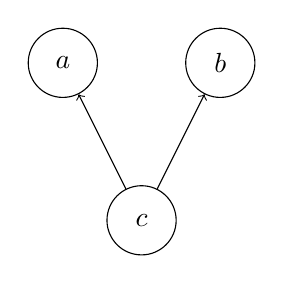
\begin{tikzpicture}[node distance=2cm]
			\node[state] (a) {$a$};
			\node[state] (b) [right of=a] {$b$};
			\node[state] (c) [below of=a, xshift=1cm] {$c$};

			\path[<-] (a) edge node {} (c);
			\path[<-] (b) edge node {} (c);
		\end{tikzpicture}
		\caption{The dependency graph of the statement ``c = a + b + 1;''}
	\end{subfigure}
	\quad
	\begin{subfigure}[b]{0.4\textwidth}
		\centering
		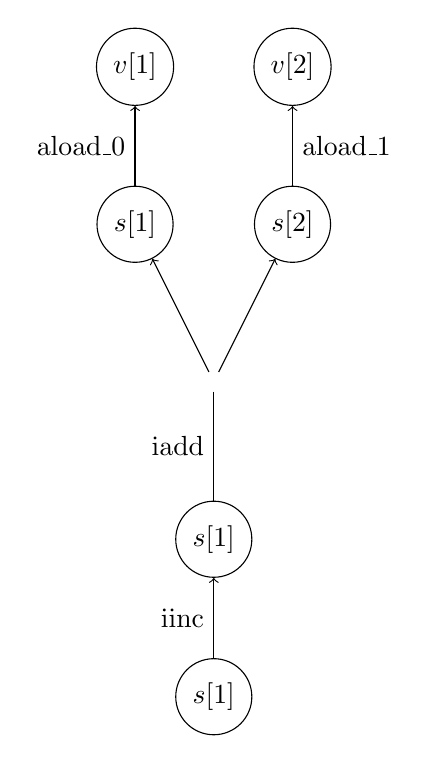
\begin{tikzpicture}[node distance=2cm]
			\node[state] (v1) {$v[1]$};
			\node[state] (s1) [below of=v1] {$s[1]$};
			\node[state] (v2) [right of=v1] {$v[2]$};
			\node[state] (s2) [below of=v2] {$s[2]$};
			\node (joint) [below of=s1, xshift=1cm] {};
			\node[state] (ns1) [below of=joint] {$s[1]$};
			\node[state] (ns2) [below of=ns1] {$s[1]$};

			\path[<-]
				(v1) edge node[left] {aload\_0} (s1)
				(v2) edge node[right] {aload\_1} (s2)
				(ns1) edge node[left] {iinc} (ns2)
				(s1) edge (joint)
				(s2) edge (joint);
			\path[-]
				(joint) edge node[left] {iadd} (ns1);
		\end{tikzpicture}
		\caption{The dependency graph of the compiled statement ``c = a + b;''}
	\end{subfigure}
	\caption{}
	\label{fig:dependency-graph-examples}
\end{figure}



Now we rewrite the program a little bit:

\begin{lstlisting}[title={Example 2}, label=code:example-2]
public void run(X, Y, Z) {
	int a = datastore.read(X);
	int b = datastore.read(Y);

	int c = a + b + 1;
	datastore.write(Z, c);
}
\end{lstlisting}

\paragraph{Identify VXE API and introduce the data label}\hfill

For oridinary programs we will see a dependency graph with \emph{a} dependening on
both \emph{datastore} and \emph{X}.  But in VXE, \emph{a} only depends on
\emph{X} but the node representing \emph{a} will be marked with a tuple (\emph{key,
version}) which designates the value that is read from the datastore.  The value
of the \emph{key} in this tuple will be replaced with the exact value of
\emph{X} at runtime.  If we execute the method with parameters $X_0, Y_0, Z_0$,
the dependency graph in Figure~\ref{fig:dependency-graph-example-for-vxe-a} can be
obtained.

\begin{figure}[htb]
	\centering
	\begin{subfigure}[b]{0.4\textwidth}
		\centering
		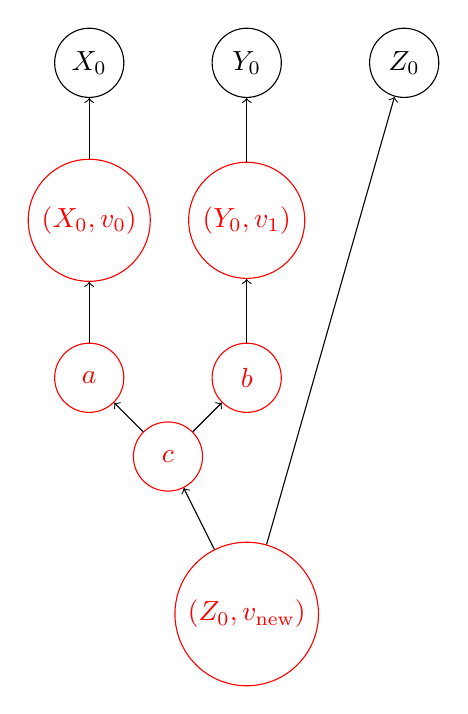
\begin{tikzpicture}[node distance=2cm]
			\node[state] (X0) {$X_0$};
			\node[state] (Y0) [right of=X0] {$Y_0$};
			\node[state] (Z0) [right of=Y0] {$Z_0$};
			\node[state] (alabel) [below of=X0, color=red] {$(X_0, v_0)$};
			\node[state] (blabel) [below of=Y0, color=red] {$(Y_0, v_1)$};
			\node[state] (a) [below of=alabel, color=red] {$a$};
			\node[state] (b) [below of=blabel, color=red] {$b$};
			\node[state] (c) [below of=a, color=red, xshift=1cm, yshift=1cm] {$c$};
			\node[state] (clabel) [below of=c, color=red, xshift=1cm] {$(Z_0,
			v_{\text{new}})$};

			\path[<-]
			(X0) edge (alabel)
			(Y0) edge (blabel)
			(alabel) edge (a)
			(blabel) edge (b)
			(a) edge (c)
			(b) edge (c)
			(c) edge (clabel)
			(Z0) edge (clabel);
		\end{tikzpicture}
		\caption{Example of a complete dependency graph for VXE}
		\label{fig:dependency-grpah-example-for-vxe-a}
	\end{subfigure}
	\quad
	\begin{subfigure}[b]{0.4\textwidth}
		\centering
		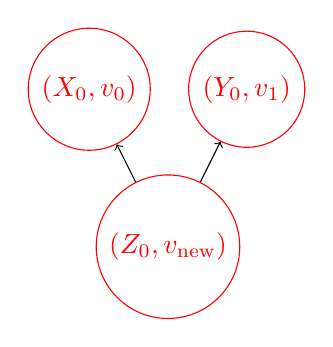
\begin{tikzpicture}[node distance=2cm]
			\node[state] (alabel) [color=red] {$(X_0, v_0)$};
			\node[state] (blabel) [right of=alabel, color=red] {$(Y_0, v_1)$};
			\node[state] (clabel) [below of=alabel, color=red, xshift=1cm] {$(Z_0,
			v_{\text{new}})$};

			\path[<-]
			(alabel) edge (clabel)
			(blabel) edge (clabel);
		\end{tikzpicture}
		\caption{Example of a compressed dependency graph for VXE}
		\label{fig:dependency-grpah-example-for-vxe-b}
	\end{subfigure}
\end{figure}


Basically the graph can be interpreted as ``the value of data at $Z_0$, whose
version is $v_{\text{new}}$, depends on the data at $X_0$ and $Y_0$, and the
corresponding versions are $v_0$ and $v_1$'', and we can futher compress it to
Figure~\ref{fig:dependency-graph-example-for-vxe-b}.

\begin{lstlisting}[]
public void run(X, Y, Z) {
	int a = datastore.read(X);
	int b = Y;

	int c = a + b + 1;
	datastore.write(Z, c);
}
\end{lstlisting}

For ordinary programs these two programs should have similar data dependency
graphs except that $b$ also depends on \emph{datastore} in the former.  In VXE,
however, they are quite different.

\challenge{For the label system to identify the VXE datastore API and get the
correct version of the },

\paragraph

\end{document}
